%\subsection{Exponential families}
%
%\begin{frame}{Exponential families}
%  \begin{itemize}[<+->]
%    \item For the mean-field variational method, suppose that each complete conditional is in the exponential family:
%    \[
%      p(\bz^{(j)}|\bz_{-j},\by) = h(\bz^{(j)})\exp \big(\eta_j(\bz_{-j},\by)\cdot \bz^{(j)} - A(\eta_j) \big).
%    \]
%    \item Then, from \eqref{eq:meanfieldsoln}, 
%    \begin{align*}
%      \tilde q_j(\bz^{(j)}) &\propto \exp\big(\E_{-j}[\log p(\bz^{(j)}|\bz_{-j},\by)]\big) \\
%      &= \exp \Big(\log h(\bz^{(j)}) + \E [\eta_j(\bz_{-j},\by)] \cdot \bz^{(j)} - \E [ A(\eta_j) ] \Big) \\
%      &\propto h(\bz^{(j)})\exp \Big(\E [\eta_j(\bz_{-j},\by)] \cdot \bz^{(j)} \Big)
%    \end{align*}
%    is also in the same exponential family.
%    \item C.f. Gibbs conditional densities.
%    \item \textbf{ISSUE}: What if not in exponential family?  Importance sampling or Metropolis sampling.
%  \end{itemize}
%\end{frame}

\begin{frame}{Non-convexity of ELBO}
  \vspace{-4pt}
  \begin{figure}
    \only<1|handout:0>{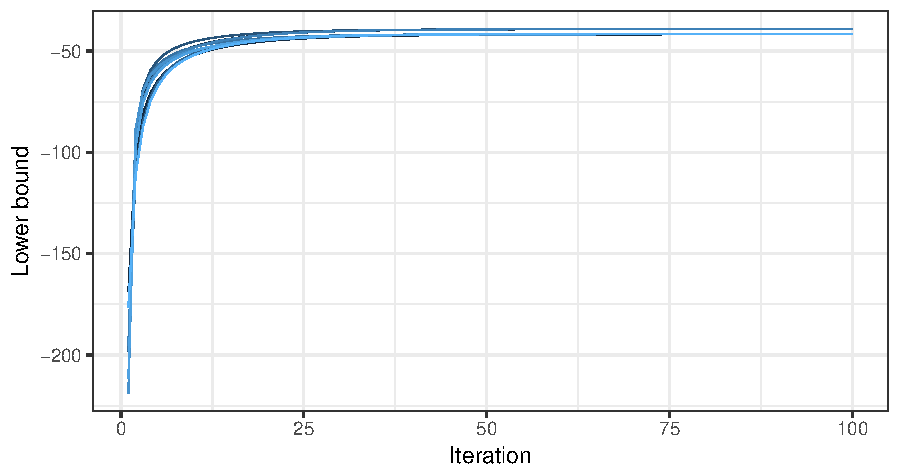
\includegraphics[scale=0.75]{figure/elbo_local_1}}
    \only<2>{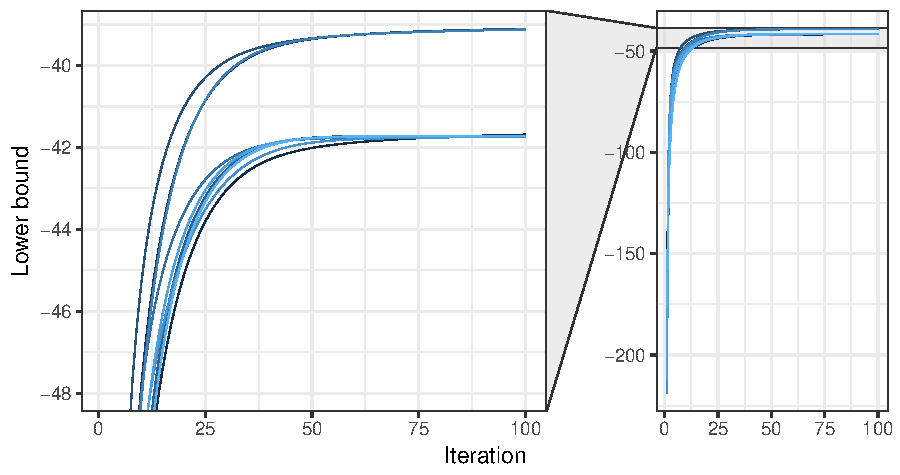
\includegraphics[scale=0.75]{figure/elbo_local_2}}
  \end{figure}
  \vspace{-8pt}
  \begin{itemize}
    \item CAVI only guarantees converges to a local optimum.
    \item Multiple local optima may exist.
  \end{itemize}
\end{frame}

\subsection{Zero-forcing vs Zero-avoiding}

\begin{frame}{Zero-forcing vs Zero-avoiding}
  \begin{itemize}
    \item Back to the KL divergence:
    \[
      \KL(q \Vert p) = \int \log \frac{q(\bz)}{p(\bz|\by)} q(\bz) \d\bz
    \]
    \item $\KL(q \Vert p)$ is large when $p(\bz|\by)$ is close to zero, unless $q(\bz)$ is also close to zero (\emph{zero-forcing}).
    \item What about other measures of closeness? \pause For instance,
    \[
      \KL(p \Vert q) = \int \log \frac{p(\bz|\by)}{q(\bz|\by)} p(\bz|\by) \d\bz.
    \]
    \item This gives the Expectation Propagation (EP) algorithm. 
    \item It is \emph{zero-avoiding}, because $\KL(p\Vert q)$ is small when both $p(\bz|\by)$ and $q(\bz)$ are non-zero.
  \end{itemize}
%  Converges to a solution, but not the overall best solution. Forward KL == EP.
\end{frame}

\begin{frame}{Zero-forcing vs Zero-avoiding (cont.)}
  \vspace{-17pt}
  \begin{figure}[t]
  \centering\hspace{-20pt}
  \only<1|handout:0>{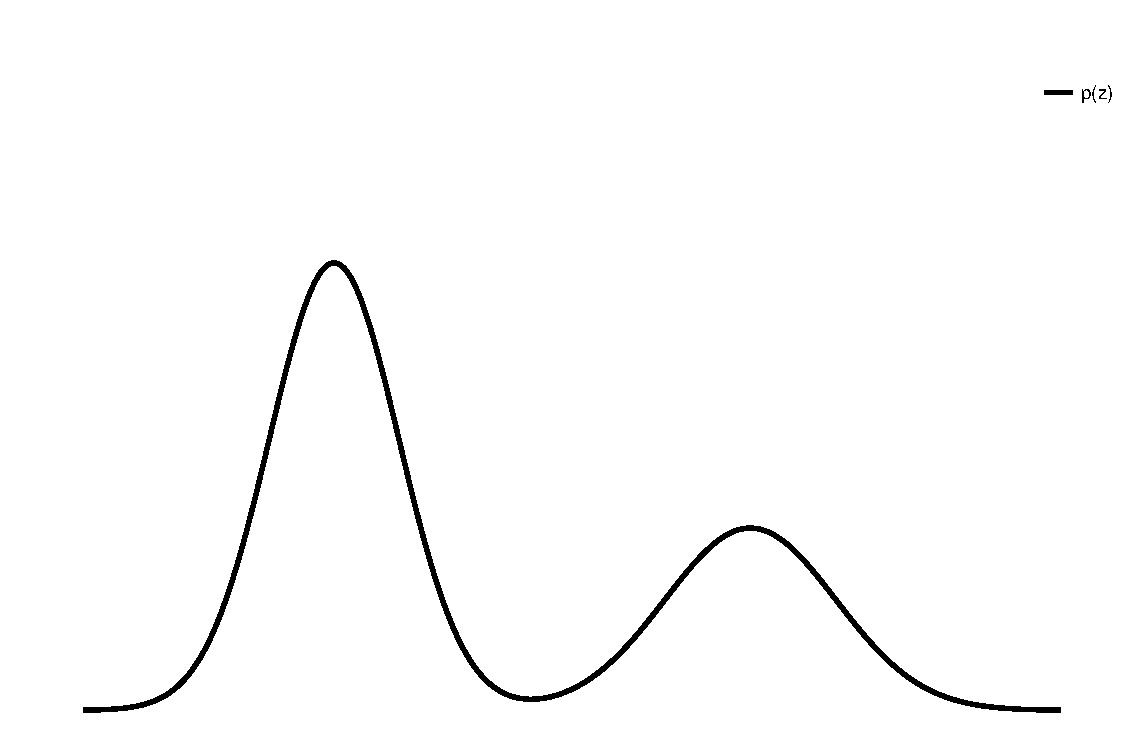
\includegraphics[scale=0.65]{figure/zero_force_1}}
  \only<2|handout:1>{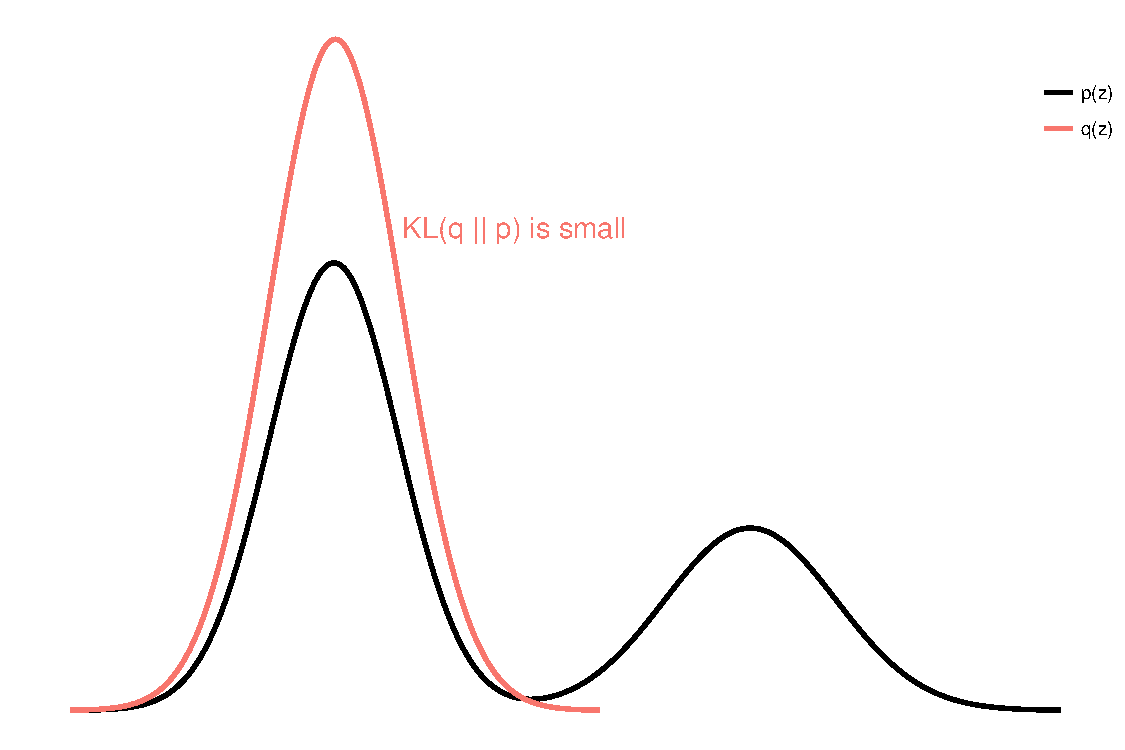
\includegraphics[scale=0.65]{figure/zero_force_2}}
  \only<3|handout:2>{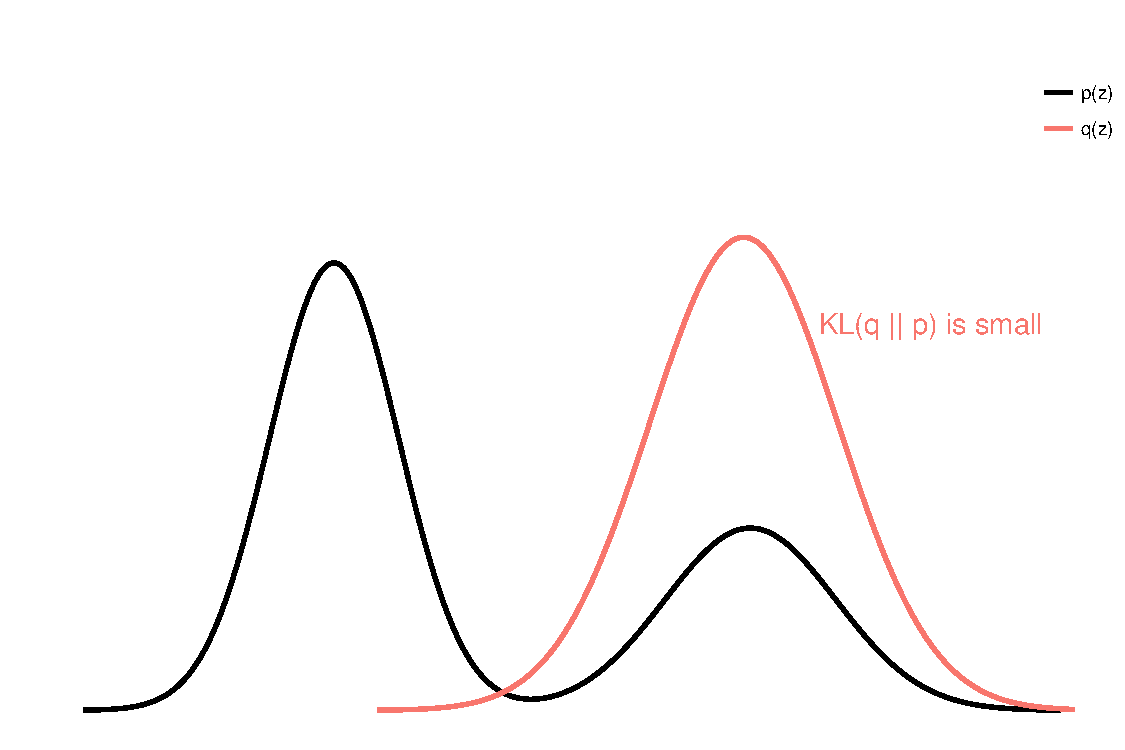
\includegraphics[scale=0.65]{figure/zero_force_3}}
  \only<4|handout:3>{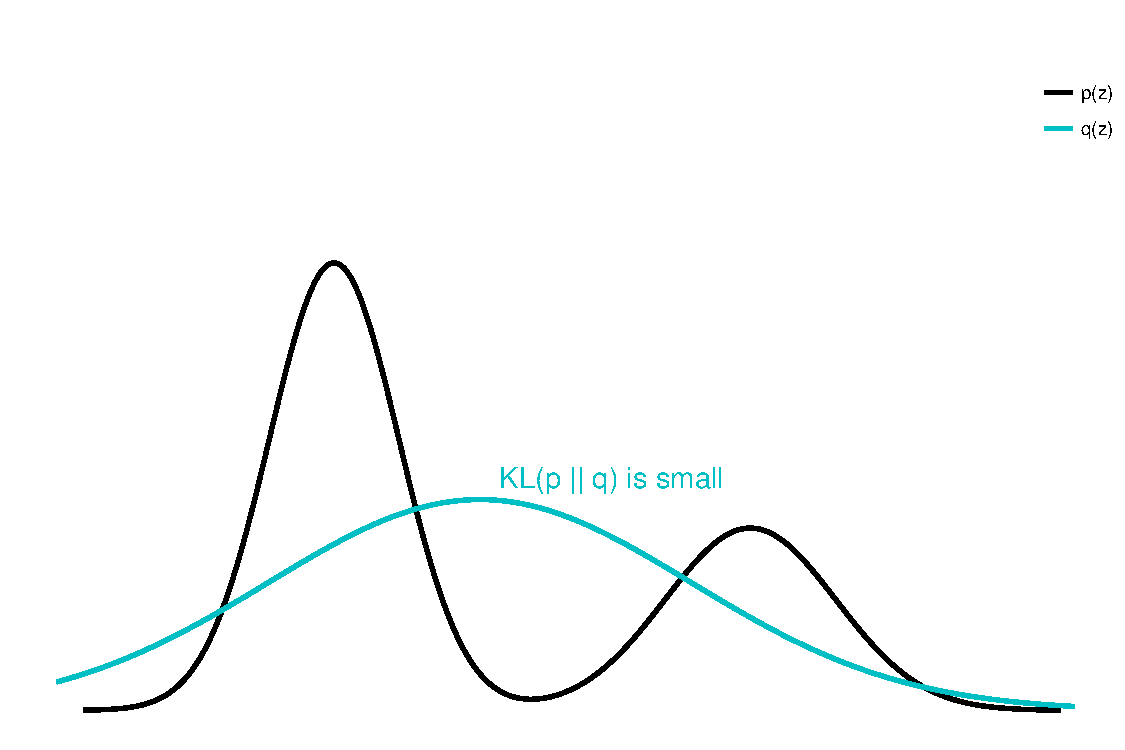
\includegraphics[scale=0.65]{figure/zero_force_4}}      
\end{figure}

\end{frame}

\subsection{Quality of approximation}

\begin{frame}{Distortion of higher order moments}
  \vspace{-11pt}
  \begin{figure}[t]
    \centering\hspace{-16pt}
    \only<1|handout:0>{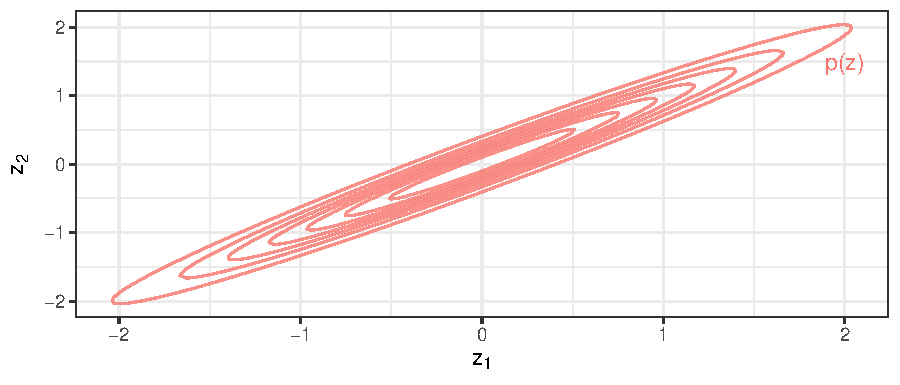
\includegraphics[scale=0.7]{figure/distorted_mean_1}}
    \only<2->{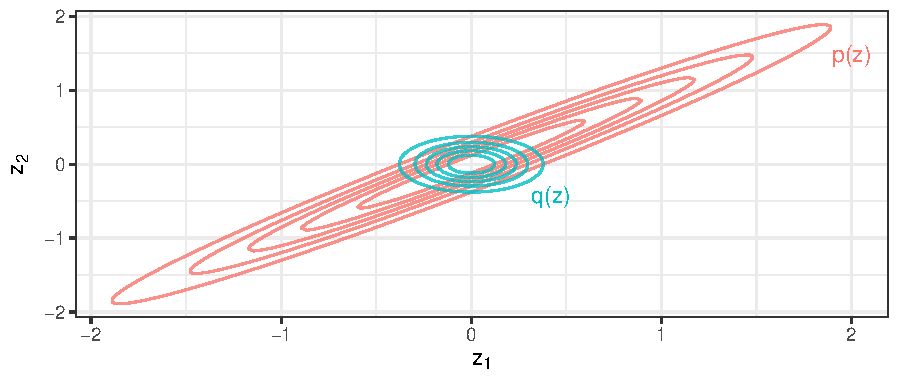
\includegraphics[scale=0.7]{figure/distorted_mean_2}}
  \end{figure}
  \vspace{-10pt}
  \begin{itemize}[<+->]
    \item Consider $\bz = (z_{1}, z_{2})^\top \sim \N_2( \bmu, \bPsi^{-1})$, $\Cov(z_1,z_2) \neq 0$.
    \item Approximating $p(\bz)$ by $q(\bz) = q_1(z_1)q_2(z_2)$ yields
    \[
      \tilde q_1(z_1) = \N(z_1|\mu_1,\psi_{11}^{-1}) \ \text{ and } \ \tilde q_2(z_2) = \N(z_2|\mu_2,\psi_{22}^{-1})
    \]
    and by definition, $\Cov(z_1,z_2) = 0$ under $\tilde q$.
    \item This leads to underestimation of variances (widely reported in the literature---\cite{zhao2013}).
  \end{itemize}
\end{frame}

\begin{frame}[label=quality]{Quality of approximation}
%  \blfootnote{\fullcite{gunawardana2005convergence}}
  \begin{itemize}[<+->]
    \item Variational inference converges to a different optimum than ML, except for certain models (\cite{gunawardana2005convergence}).
    \item But not much can be said about the quality of approximation.
    \item Statistical properties not well understood---what is its statistical profile relative to the exact posterior?
    \item Speed trumps accuracy?
  \end{itemize}
  \vspace{10pt}
  \centering
  \onslide<4->{
  \hspace{-13pt}
  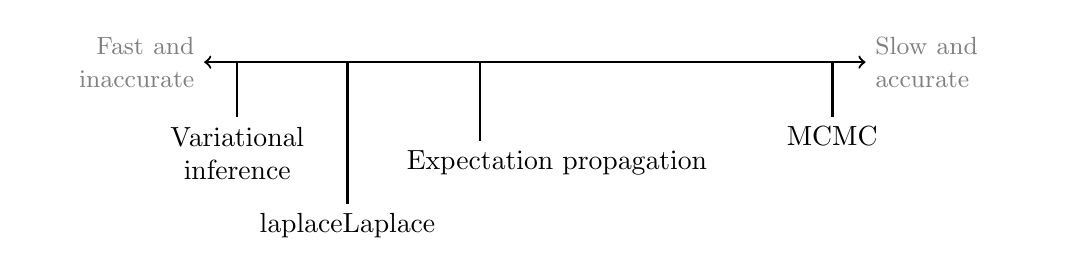
\begin{tikzpicture}[xscale=1.4]
  	\draw [<->,thick] (0,0) -- (6,0);
  	\node[left,text width=2cm,align=right] at (0,0) {\color{gray}\small Fast and inaccurate};
 	\node[right,text width=2cm,align=left] at (6,0) {\color{gray}\small Slow and accurate};
  	\draw[thick] (0.3,0) -- (0.3, -0.7);
  	\node[align=center,text width=2cm,below] at (0.3,-0.7) {Variational inference};
  	\draw[thick] (5.7,0) -- (5.7, -0.7);
  	\node[align=left,text width=2cm,below] at (6,-0.7) {MCMC};  	
  	\draw[thick] (1.3,0) -- (1.3, -1.8);
  	\node[align=center,below] at (1.3,-1.8) {\hyperlink{laplace}{Laplace}};  	  
  	\draw[thick] (2.5,0) -- (2.5, -1);	
  	\node[align=center,below] at (3.2,-1) {Expectation propagation};
  \end{tikzpicture}
  }
  
%  \begin{textblock*}{3cm}(.982\textwidth,1.04\textheight)%
%    \hyperlink{laplace}{\beamerbutton{back}}      
%  \end{textblock*}
\end{frame}

%\subsection{Advanced topics}
%
%\begin{frame}{Advanced topics}
%  \begin{itemize}
%    \item<1-> Local variational bounds 
%    \begin{itemize}
%      \item Not using the mean-field assumption.
%      \item Instead, find a bound for the marginalising integral $\cI$.
%      \item Used for Bayesian logistic regression as follows:
%      \[
%        I = \int \expit(x^\top\beta) p(\beta) \d\beta \geq \int f(x^\top\beta,\xi) p(\beta) \d\beta.
%      \]
%    \end{itemize}
%    \item<2-> Stochastic variational inference
%    \begin{itemize}
%%      \item VI on its own doesn't offer much computational advantages.
%      \item Use ideas from stochastic optimisation---gradient based improvement of ELBO from subsamples of the data.
%      \item Scales to massive data.
%    \end{itemize}
%    \item<3-> Black box variational inference
%    \begin{itemize}
%      \item Beyond exponential families and model-specific derivations.
%    \end{itemize}
%  \end{itemize}
%\end{frame}
